\documentclass[11pt,a4paper]{article}
\usepackage{iftex}
\ifPDFTeX
  \usepackage[T1]{fontenc}
  \usepackage[utf8]{inputenc}
  \usepackage{lmodern}
  \renewcommand{\familydefault}{\sfdefault}
\else
  \usepackage{fontspec}
  \setmainfont{lmsans10-regular}[Extension=.otf,BoldFont=lmsans10-bold,ItalicFont=lmsans10-oblique,BoldItalicFont=lmsans10-boldoblique]
  \setmonofont{lmmono10-regular}[Extension=.otf]
\fi
\usepackage{babel}
\babelprovide[import,main]{french}
\usepackage[a4paper,margin=1.9cm,top=1.7cm,bottom=1.8cm]{geometry}
\usepackage{amsmath,amssymb,mathtools}
\usepackage{booktabs,array,tabularx}
\usepackage{microtype}
\usepackage[table]{xcolor}
\usepackage{tcolorbox}
\usepackage{enumitem}
\usepackage{fancyhdr,lastpage}
\usepackage{titlesec}
\usepackage{graphicx}
\usepackage{caption}
\captionsetup{font={small,color=Muted},labelfont={bf,color=Forest},skip=3pt}
\usepackage{hyperref}
\definecolor{Forest}{HTML}{174F43}
\definecolor{Sage}{HTML}{EDF2E6}
\definecolor{Ink}{HTML}{243C35}
\definecolor{Muted}{HTML}{65756A}
\definecolor{Amber}{HTML}{80633D}
\definecolor{Sand}{HTML}{FBF1E3}
\hypersetup{colorlinks=true,linkcolor=Forest,urlcolor=Forest,pdfauthor={Projet Clair},pdflang={fr-FR}}
\color{Ink}
\setlength{\parindent}{0pt}
\setlength{\parskip}{6pt}
\setlength{\headheight}{15pt}
\setlength{\emergencystretch}{2em}
\linespread{1.08}
\setlist[itemize]{leftmargin=1.3em,itemsep=3pt,topsep=4pt}
\setlist[enumerate]{leftmargin=1.5em,itemsep=4pt,topsep=4pt}
\titleformat{\section}{\Large\bfseries\color{Forest}}{\thesection}{.65em}{}
\titleformat{\subsection}{\normalsize\bfseries\color{Forest}}{}{0pt}{}
\titlespacing*{\section}{0pt}{9pt}{8pt}
\titlespacing*{\subsection}{0pt}{9pt}{3pt}
\newtcolorbox{keybox}{colback=Sage,colframe=Sage,boxrule=0pt,arc=3mm,left=3mm,right=3mm,top=2mm,bottom=2mm}
\newtcolorbox{limitbox}{colback=Sand,colframe=Sand,boxrule=0pt,arc=3mm,left=3mm,right=3mm,top=2mm,bottom=2mm}
\newcommand{\E}{\mathbb E}
\newcommand{\Var}{\operatorname{Var}}
\newcommand{\Cov}{\operatorname{Cov}}
\newcommand{\G}{\operatorname{Gamma}}
\newcommand{\Pois}{\operatorname{Poisson}}
\newcommand{\NB}{\operatorname{NB2}}
\newcommand{\RMSEP}{\operatorname{RMSEP}}
\newcommand{\MSEP}{\operatorname{MSEP}}
\newcommand{\smallnote}[1]{{\small\color{Muted}#1}}
\pagestyle{fancy}
\fancyhf{}
\fancyhead[L]{\small\bfseries\color{Forest}CLAIR / NOTE MÉTHODOLOGIQUE}
\fancyhead[R]{\small\color{Muted}Version du 12 novembre 2026}
\fancyfoot[L]{\footnotesize\color{Muted}Méthodes implémentées, résultats mesurés, limites explicites.}
\fancyfoot[R]{\footnotesize\color{Forest}\thepage\,/\,\pageref{LastPage}}
\renewcommand{\headrulewidth}{0pt}
\renewcommand{\footrulewidth}{0pt}
\hypersetup{pdftitle={Clair — Provisionnement : Chain-Ladder, Mack et bootstrap}}
\begin{document}
{\small\color{Muted}\textbf{NOTE 02}\quad PROVISIONNEMENT ET INCERTITUDE}
\vspace{5mm}

{\fontsize{27}{31}\selectfont\bfseries\color{Forest}Du triangle observé\par au développement futur.}

{\large Chain-Ladder, erreur de prédiction de Mack,\par bootstrap ODP et validation rétrospective.}
\vspace{3mm}

\begin{keybox}
\textbf{Objectif.} Estimer le développement restant des sinistres déjà survenus, expliquer les hypothèses et rendre visible l'incertitude. Le projet comprend un moteur Python indépendant d'une interface métier locale Streamlit/Plotly.
\end{keybox}

\section*{Ce qui est effectivement réalisé}
\begin{itemize}
\item Lecture et contrôle d'un triangle annuel ; observations et projections conservées séparément.
\item Facteurs Chain-Ladder, ultimes et provisions par origine.
\item RMSEP de Mack, avec covariance interannuelle dans le total.
\item Bootstrap ODP de bibliothèque avec correction déterministe des leviers et processus Gamma signé, distinct du bootstrap Mack.
\item Comparaison à une implémentation externe, diagonales connues masquées, tests actuariels et tests de l'interface.
\end{itemize}

\subsection*{Référence du cours reproduite}
\begin{center}
\begin{tabular}{lr}
\toprule
Développement futur estimé & \textbf{18\,680\,847,77} \\
Erreur de prédiction Mack (RMSEP) & \textbf{2\,447\,093,03} \\
RMSEP / estimation & \textbf{13,1\,\%} \\
\bottomrule
\end{tabular}
\end{center}
\smallnote{Montants dans l'unité du fichier du cours, qui ne précise pas une devise. La RMSEP n'est ni une marge à ajouter automatiquement ni une probabilité d'insuffisance.}

\begin{limitbox}
\textbf{Périmètre de la V1.} Queue fixée à 1, aucune inflation ni actualisation appliquée. La reproduction des références vérifie les calculs ; l'adéquation des hypothèses au portefeuille nécessite une revue actuarielle. Schnieper et inflation restent des extensions.
\end{limitbox}

\smallnote{Version moteur : \texttt{reserving-v1}. Référence externe : \texttt{chainladder 0.10.1}, avec pondération par volume et variance finale de Mack. Application livrée pour une démonstration locale ; aucun déploiement public effectué.}

\newpage
\section{Triangle et estimation Chain-Ladder}
\subsection*{Données disponibles à la date d'arrêté}
En indices mathématiques $i,j\in\{1,\ldots,n\}$, $C_{i,j}$ est le montant cumulé pour l'origine $i$ à l'âge $j$. On observe les cellules $i+j\leq n+1$. Le dernier âge connu de l'origine $i$ est $k_i=n+1-i$.

Les montants incrémentaux sont
\[
X_{i,1}=C_{i,1},\qquad X_{i,j}=C_{i,j}-C_{i,j-1}\quad(j\geq2).
\]
La V1 exige des cumuls observés strictement positifs et une géométrie triangulaire complète. Les cellules futures sont \texttt{NA}, jamais des zéros interprétés comme des observations. Les reprises négatives sont autorisées pour Mack si les cumuls restent positifs.

\subsection*{Facteurs pondérés par volume}
Pour $j=1,\ldots,n-1$ :
\[
\boxed{\widehat f_j=\frac{\sum_{i=1}^{n-j}C_{i,j+1}}{\sum_{i=1}^{n-j}C_{i,j}}.}
\]
Toutes les paires observées admissibles contribuent au facteur. La projection est
\[
\widehat C_{i,j+1}=\widehat f_j\widehat C_{i,j},\qquad
\boxed{\widehat U_i=C_{i,k_i}\prod_{j=k_i}^{n-1}\widehat f_j.}
\]
On déduit
\[
\boxed{\widehat R_i=\widehat U_i-C_{i,k_i},\qquad
\widehat R=\sum_{i=1}^n\widehat R_i.}
\]
Le facteur de queue est fixé à 1 : $C_{i,n}$ est supposé représenter le terme du développement retenu. Aucun développement supplémentaire au-delà de cet âge n'est estimé dans cette version.

\begin{figure}[htbp]
\centering
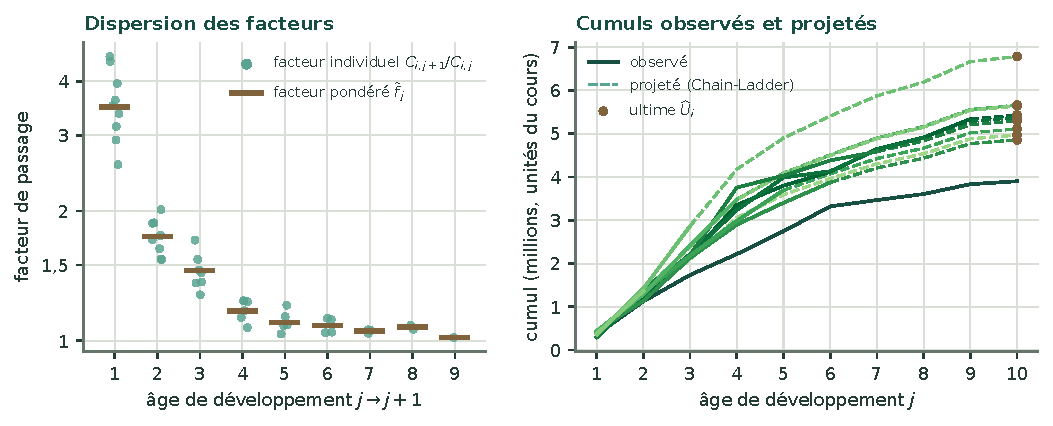
\includegraphics[width=\linewidth]{figures/fig_triangle.pdf}
\caption{Triangle du cours. À gauche, chaque facteur de passage observé (points) et le facteur pondéré par volume $\widehat f_j$ (trait) ; la dispersion augmente aux âges élevés, où peu d'origines contribuent. À droite, cumuls observés (trait plein) et projetés (pointillés) jusqu'à l'ultime $\widehat U_i$.}\label{fig:triangle}
\end{figure}

\subsection*{L'interprétation dépend de la nature du triangle}
\begin{itemize}
\item \textbf{Paiements :} ultime estimé moins déjà payé = montant estimé restant à payer.
\item \textbf{Charges encourues :} ultime estimé moins charge actuelle = développement futur de charge. Ce montant n'est pas le reste à payer total.
\item \textbf{Nature non confirmée :} l'interface emploie le libellé neutre « développement futur estimé ».
\end{itemize}

\begin{keybox}
\textbf{Contrôles métier.} Le fichier CSV contient \texttt{origin,D1,D2,...,Dn}. Les années numériques sont croissantes et consécutives. Les observations restent intactes ; le triangle projeté est un autre tableau. Nature, unité et date d'évaluation sont incluses dans l'export et dans l'empreinte du dossier.
\end{keybox}

\section{Mack : mesurer l'erreur de prédiction}
\subsection*{Hypothèses de moments}
Les origines sont supposées indépendantes. Conditionnellement à l'historique disponible :
\[
\E[C_{i,j+1}\mid\mathcal F_{i,j}]=f_jC_{i,j},\qquad
\Var(C_{i,j+1}\mid\mathcal F_{i,j})=\sigma_j^2C_{i,j}.
\]
Le modèle ne spécifie pas une loi complète de la provision. La stabilité des facteurs et de la relation variance/cumul entre origines reste une hypothèse à examiner.

Pour $m_j=n-j\geq2$ paires observées :
\[
\widehat\sigma_j^2=\frac1{m_j-1}\sum_{i=1}^{m_j}
\frac{(C_{i,j+1}-\widehat f_jC_{i,j})^2}{C_{i,j}}.
\]
La dernière transition ne dispose que d'une paire. L'approximation retenue est
\[
\widehat\sigma_{n-1}^2=\min\!\left(
\frac{(\widehat\sigma_{n-2}^2)^2}{\widehat\sigma_{n-3}^2},
\widehat\sigma_{n-2}^2,\widehat\sigma_{n-3}^2\right).
\]
Si le dénominateur est nul, le minimum est fixé à zéro. Cette convention et le besoin d'au moins quatre origines sont explicites.

\subsection*{Processus, estimation et covariance}
Posons $S_j=\sum_{l=1}^{n-j}C_{l,j}$ et $U_i=\widehat C_{i,n}$. Les composantes calculées sont
\[
V_i^{\rm proc}=U_i^2\sum_{j=k_i}^{n-1}
\frac{\widehat\sigma_j^2}{\widehat f_j^2\widehat C_{i,j}},
\]
\[
V_{ik}^{\rm param}=U_iU_k\sum_{j=\max(k_i,k_k)}^{n-1}
\frac{\widehat\sigma_j^2}{\widehat f_j^2S_j}.
\]
Par conséquent,
\[
\boxed{\MSEP_i=V_i^{\rm proc}+V_{ii}^{\rm param},\qquad
\MSEP_{\rm total}=\sum_iV_i^{\rm proc}+\sum_{i,k}V_{ik}^{\rm param}.}
\]
La RMSEP est la racine carrée de la MSEP. Les covariances sont incluses dans le total ; les écarts-types annuels ne s'additionnent pas.

\begin{figure}[htbp]
\centering
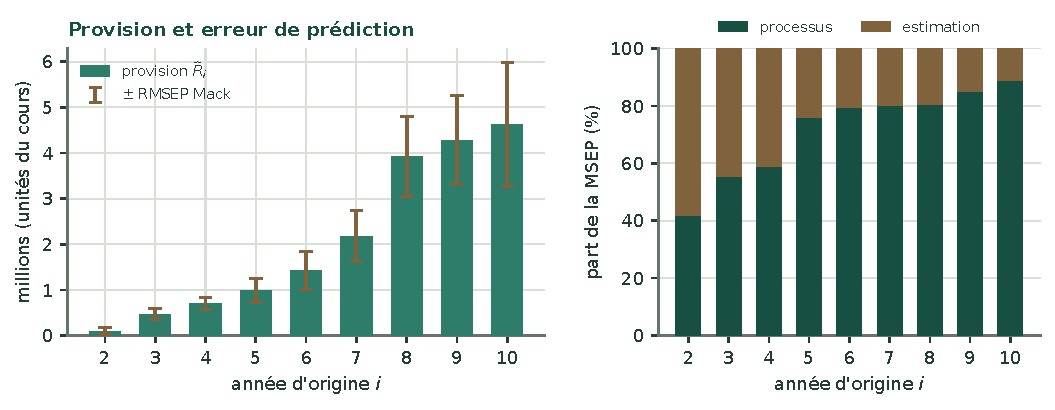
\includegraphics[width=\linewidth]{figures/fig_mack.pdf}
\caption{Erreur de prédiction de Mack sur le cours. À gauche, provision par origine et RMSEP annuelle (les écarts-types annuels ne s'additionnent pas). À droite, part de la MSEP due au processus et à l'estimation des facteurs.}\label{fig:mack}
\end{figure}

\smallnote{Sur le cours : écart-type de processus agrégé $\simeq1\,878\,290{,}22$ ; écart-type d'estimation agrégé $\simeq1\,568\,531{,}20$. Leurs \emph{variances} s'additionnent pour donner la RMSEP totale $2\,447\,093{,}03$. Une loi normale et un intervalle $R\pm1{,}96\,\RMSEP$ ne sont pas déduits automatiquement de Mack.}

\newpage
\section{Bootstrap ODP et scénarios de processus}
\subsection*{Un modèle distinct de Mack}
Le bootstrap représente les incréments par une moyenne multiplicative origine/développement $\mu_{i,j}$, avec une variance ODP $\phi\mu_{i,j}$ lorsque la moyenne est positive. Sur $N$ cellules observées et $p=2n-1$ paramètres :
\[
\widehat\phi=\frac1{N-p}\sum_{\rm obs}\frac{(X_{i,j}-\widehat\mu_{i,j})^2}{\widehat\mu_{i,j}}.
\]
Les résidus de Pearson sont ajustés par le levier $h_{i,j}$, puis centrés et rééchantillonnés :
\[
r_{i,j}=\frac{X_{i,j}-\widehat\mu_{i,j}}{\sqrt{\widehat\mu_{i,j}(1-h_{i,j})}}.
\]
Pour les observations saturées $h=1$, aucun résidu n'est estimable. Leur correction est explicitement nulle. Un correctif local du calcul de levier évite une mémoire non initialisée détectée dans la bibliothèque ; sa reproductibilité est testée.

On reconstruit les pseudo-triangles, on réestime le développement et on ajoute le processus futur. La bibliothèque utilise, pour un incrément moyen futur $m$ :
\[
\boxed{X^*=\operatorname{sign}(m)\,G,\qquad
G\sim\G\!\left(\text{forme}=\frac{|m|}{\widehat\phi},\ \text{échelle}=\widehat\phi\right).}
\]
Ici la convention est \emph{forme/échelle} : $\E[X^*]=m$ et $\Var(X^*)=\widehat\phi|m|$. Pour $m<0$, c'est une \textbf{extension Gamma signée}, au-delà de l'ODP strict à moyenne positive.

\subsection*{Résultats effectivement simulés sur le cours}
\begin{center}
\begin{tabular}{lr}
\toprule
Scénarios / graine & 5\,000 / 42 \\
Moyenne & 18\,840\,414,38 \\
Médiane & 18\,652\,950,34 \\
Écart-type & 2\,945\,899,68 \\
Quantile 95\,\% & \textbf{24\,138\,111,42} \\
Quantile 99\,\% & 26\,805\,701,39 \\
Erreur Monte-Carlo de la moyenne & 41\,661,31 \\
\bottomrule
\end{tabular}
\end{center}
\begin{figure}[htbp]
\centering
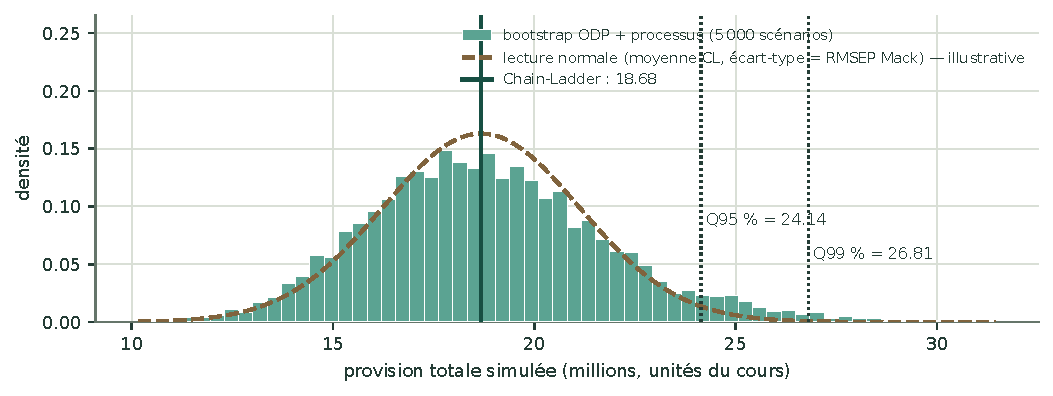
\includegraphics[width=\linewidth]{figures/fig_bootstrap.pdf}
\caption{Provision totale simulée sur le cours (bootstrap ODP et processus Gamma signé, 5\,000 scénarios, graine 42). La courbe normale construite avec la RMSEP de Mack n'est qu'un repère visuel : aucune loi n'est déduite de Mack.}\label{fig:bootstrap}
\end{figure}

\begin{limitbox}
444 scénarios sur 5\,000 contiennent des incréments futurs moyens négatifs ; ils sont conservés par le processus signé. Aucune réserve totale simulée n'est négative. Aucune simulation invalide n'est supprimée. Les quantiles sont ceux de ce modèle jusqu'au terme retenu ; ce ne sont ni des quantiles Mack ni un SCR à un an.
\end{limitbox}

\newpage
\section{Références et diagonales masquées}
\subsection*{Réconciliation avec une implémentation externe}
Les calculs ont été comparés à \texttt{chainladder 0.10.1}, avec pondération par volume, variance finale « Mack » et queue égale à 1.

\begin{center}
\small
\begin{tabularx}{\linewidth}{Xrr}
\toprule
Jeu & Développement futur & RMSEP Mack \\
\midrule
Cours & 18\,680\,847,77 & 2\,447\,093,03 \\
GenIns & 18\,680\,855,61 & 2\,447\,094,86 \\
RAA & 52\,135,23 & 26\,909,01 \\
CAS/NAIC, State Farm, ppauto & 12\,586\,821,36 & 550\,736,26 \\
\bottomrule
\end{tabularx}
\end{center}
Les écarts de réserve et de RMSEP sont inférieurs à $10^{-6}$ unité. Les facteurs et erreurs annuelles sont aussi comparés. \textbf{Le cours n'est pas exactement GenIns :} en ligne 8, colonne 3, les valeurs sont respectivement 2\,864\,494 et 2\,864\,498. La différence est conservée.

Le cas réel utilise un seul groupe, \emph{State Farm Mut Grp}, une seule branche, \emph{ppauto}, et les paiements cumulés \texttt{CumPaidLoss} : origines 1988--1997, évaluation fin 1997. Les unités CAS/NAIC restent non converties.

\subsection*{Validation rétrospective sans fuite du futur}
Trois arrêts antérieurs sont reconstruits. À chaque arrêt, on masque les données ultérieures, réestime les facteurs et prédit la diagonale suivante connue. Le ratio ci-dessous porte sur les \emph{incréments} observés/prédits.

\begin{center}
\begin{tabular}{lrrr}
\toprule
Jeu & Arrêt le plus récent & Précédent & Troisième \\
\midrule
Cours & 115,30\,\% & 109,86\,\% & 74,75\,\% \\
GenIns & 115,30\,\% & 109,86\,\% & 74,75\,\% \\
RAA & 67,35\,\% & 119,99\,\% & 116,43\,\% \\
CAS/NAIC & 86,77\,\% & 85,88\,\% & 89,53\,\% \\
\bottomrule
\end{tabular}
\end{center}
La nouvelle origine et la plus ancienne au-delà de la maturité ajustée sont exclues. Un test vérifie que modifier les observations masquées ne change pas leur propre prédiction.

\begin{figure}[htbp]
\centering
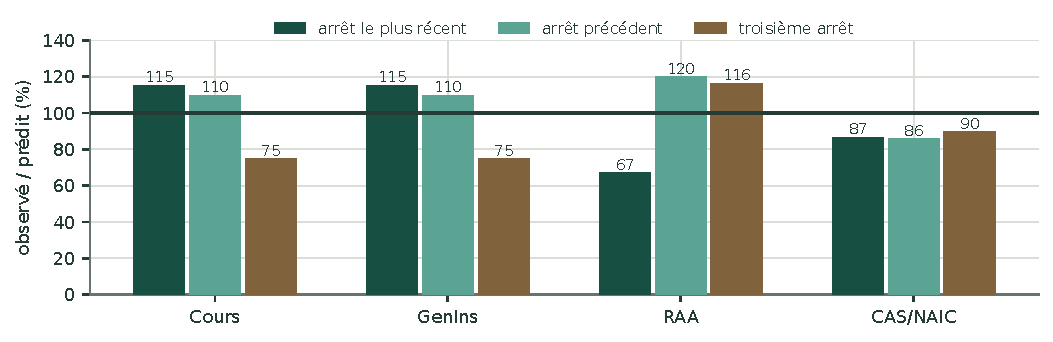
\includegraphics[width=\linewidth]{figures/fig_backtest.pdf}
\caption{Rapport observé/prédit des incréments des diagonales masquées, par jeu et par arrêt (100\,\% = prédiction exacte). Le cas CAS/NAIC est systématiquement surestimé ; les autres jeux sont instables d'un arrêt à l'autre.}\label{fig:backtest}
\end{figure}

\begin{limitbox}
Sur le cas CAS/NAIC, les ratios inférieurs à 1 indiquent une surestimation des paiements des diagonales masquées. Ces résultats sont publiés tels quels. Trois arrêts sur un triangle ne valident pas l'ultime réel, la queue de distribution ou l'usage sur d'autres portefeuilles.
\end{limitbox}

\section{Usage métier, reproductibilité et limites}
\subsection*{Fonctionnalités livrées}
\begin{itemize}
\item Interface Streamlit/Plotly : source ou CSV, nature, unité et date d'évaluation ; triangle observé/projeté, résultats par origine, facteurs et diagnostics.
\item Simulation à graine explicite ; histogramme et quantiles, diagnostics signés et stabilité Monte-Carlo par lots.
\item Exports JSON et CSV, avec source, hypothèses, version du moteur et empreinte des données/métadonnées.
\item Changer de triangle invalide l'affichage du bootstrap précédent. Les fichiers importés restent en mémoire de session ; aucun enregistrement automatique de données client.
\end{itemize}

\subsection*{Contrôles et références réellement exécutés}
Le projet comporte \textbf{24 tests réussis} : réconciliation des références, covariance, échelle, préservation des observations, erreurs de format et de géométrie, correction des leviers, reproductibilité, risque de processus, provision nulle renvoyée en NaN par la bibliothèque, reproduction des statistiques publiées du bootstrap, absence de fuite et parcours Streamlit.

La comparaison exécutée utilise l'implémentation Python indépendante de la bibliothèque \texttt{chainladder}. Un script R facultatif est fourni avec les mêmes options, mais \textbf{n'a pas été exécuté}, car \texttt{Rscript} est absent de l'environnement de réalisation. Une valeur RAA publiée avec variance finale log-linéaire ne doit pas être comparée sans harmoniser ce choix.

\subsection*{Ce qui reste à valider avant une utilisation compagnie}
\begin{itemize}
\item Homogénéité des données, définition payé/encouru, échelle monétaire et périmètre brut/net de réassurance.
\item Stabilité des cadences, indépendance des origines, effets calendaires et changements de gestion.
\item Développement au-delà du dernier âge ; le facteur de queue égal à 1 est actuellement une hypothèse fixe.
\item Inflation, actualisation et risque de modèle ; aucun de ces éléments n'est implicitement couvert par la RMSEP ou le bootstrap.
\end{itemize}

\smallnote{Schnieper exige de vrais triangles de nouveaux sinistres $N$, de révisions $D$ et des expositions $E$. Le triangle cumulé seul ne permet pas d'identifier cette décomposition. L'inflation devrait être traitée sur les incréments par année calendaire, avec indices et scénarios documentés. Ces deux modules sont des extensions prévues, pas des résultats livrés.}

\subsection*{Code, méthodes et sources}
\small
\begin{itemize}[itemsep=2pt]
\item \href{https://github.com/kelian19/assurance-provisionnement}{Dépôt : kelian19/assurance-provisionnement}. Voir \texttt{docs/METHODOLOGIE.md}, \texttt{reports/validation.json} et \texttt{reports/RESULTATS.md}.
\item \href{https://nicolasbaradel.fr/enseignement/ressources/R/donneesMACK.txt}{Triangle du cours fourni} ; Nicolas Baradel, \emph{Mathématiques de l'assurance dommages}, version du 8 septembre 2026, p. 25--69.
\item \href{https://mages.github.io/ChainLadder/articles/ChainLadder.html}{ChainLadder R : méthodes et références}.
\item \href{https://chainladder-python.readthedocs.io/main/library/generated/chainladder.BootstrapODPSample.html}{Chainladder Python : BootstrapODPSample}.
\item \href{https://casact.github.io/raw_package/reference/NAIC.html}{CAS/NAIC : documentation des données Schedule P}.
\end{itemize}
\end{document}

ewpage
